\documentclass[a4paper, 12pt]{exam}

%\usepackage{mathpazo}
\usepackage[onehalfspacing]{setspace}
\usepackage{graphicx}
\usepackage{amsmath, amssymb, amsfonts}
\usepackage[table]{xcolor}
\usepackage{gensymb}
\usepackage[]{booktabs}
\usepackage[utf8]{inputenc}
\usepackage{array}
\usepackage{setspace}
\usepackage{xhfill}
\usepackage{enumitem}
\usepackage{multicol}
\usepackage{mathtools}
%\usepackage{background} %Package for adding a watermark

%\backgroundsetup{scale = 1, angle = 0, firstpage = false, opacity=0.1, contents=\includegraphics{Watermark}}

\newcommand{\dho}{\partial}
\newcommand{\cuspac}{\hspace{0.5cm}}
\newcommand{\longspac}{\hspace{1cm}}
\newcommand{\tripdot}{\cdot \cdot \cdot}


\mathtoolsset{showonlyrefs}

\title{
	{Answers to TTC Subsystem Test} \\
	\textbf{\large Team Ananat Recruitment Test}\\
	\vspace{0.75cm}
	%\includegraphics[scale = 0.5]{Watermark}
}
\date{28th January, 2024}
\author{Pranav Chandra N.V \\ 2023AAPS0013P}


\begin{document}
	\maketitle
	\newpage
	\begin{questions}
		\question \textbf{ Rx antenna design.}
		\begin{parts}
			\part \textbf{Type of antenna and dimensions.}
			
			There are many styles of antennae (as mentioned in the website https://www.antenna-theory.com/antennas.php), but the important part is that each of these antennae vary in complexity and viability for Ishan.
			
			Given that the only materials he has are copper pipes and sheets, it would be wise to create a dipole antenna. Specifically, either a half-wavelength dipole or quarter-wavelength monopole antenna or folded dipole antenna. (In descending order of preference).
			
			This preference order has been chosen since the dipole and monopole antennae are some of the easiest to build. Additionally, they have the ability to continue to broadcast omnidirectionally, allowing Ishan to communicate with the satellite even if the exact position of it is unknown.	
			
			The next important factor to consider is ease of construction. monopole and dipole atennae are some of the easist to construct since they're essentially just copper rods. \textbf{However} the folded dipole antenna will require more precise folding to get it to do what we want, making it rank last on the list.
			
			Overall, it is probably in Ishan's best interest to make a quarter-wavelength monopole antenna or a half-wavelength dipole antenna, in that order. This is to ensure maximum simplicity of building and best performance.
			
			\part \textbf{Connection of coaxial cable.}
			
			The center-fed connection of the coaxial cable is likely the best option. This is because it's easier to attach and is less prone to changing due to external factors.
			
			\part \textbf{Gain plot of antenna:}
			\begin{figure}
				content...
			\end{figure}
			
			\part \textbf{Diameter of copper rods:}	
			
		\end{parts}
		
		\newpage
		
		\question \textbf{Transmission question}
		\begin{parts}
			\part \textbf{Why do we send data like this?}
			
				Data transmission is done in packets rather than a continuous stream for a variety of reasons as follows:
				\begin{itemize}
					\item Error correction  - Having the error correction at the end of each packet allows us to check, packet by packet, if there's any particular error and immediately try to correct it.
					
					\item Tracking of data - When sending data in a continuous stream, we have to have markers at continuous intervals to see if a message has been interrupted. However, if we send data as packets, we are able to quickly figure out when and where transmission has stopped as well as restart transmission from the last ended point more effectively,
					
					\item Data resilience - This is basically the concept of being able to recheck transmitted data more effectively in a packet than as a continuous stream. We can more easily work in error correction protocols into shorter packets of data than in larger streams.
				\end{itemize}
				
				\part \textbf{Implementation of a CRC for "c"}
				\begin{enumerate}
					\item Convert "c" to hex $\rightarrow$ c = 1100
					\item Append zeroes to the code to shift it by the degree 3 polynomial. $\rightarrow$ 1100000
					\item Perform polynomial division with $x^3 + x^2 + 1$ which is written as $1101$.
					\begin{figure}[h!]
						\centering
						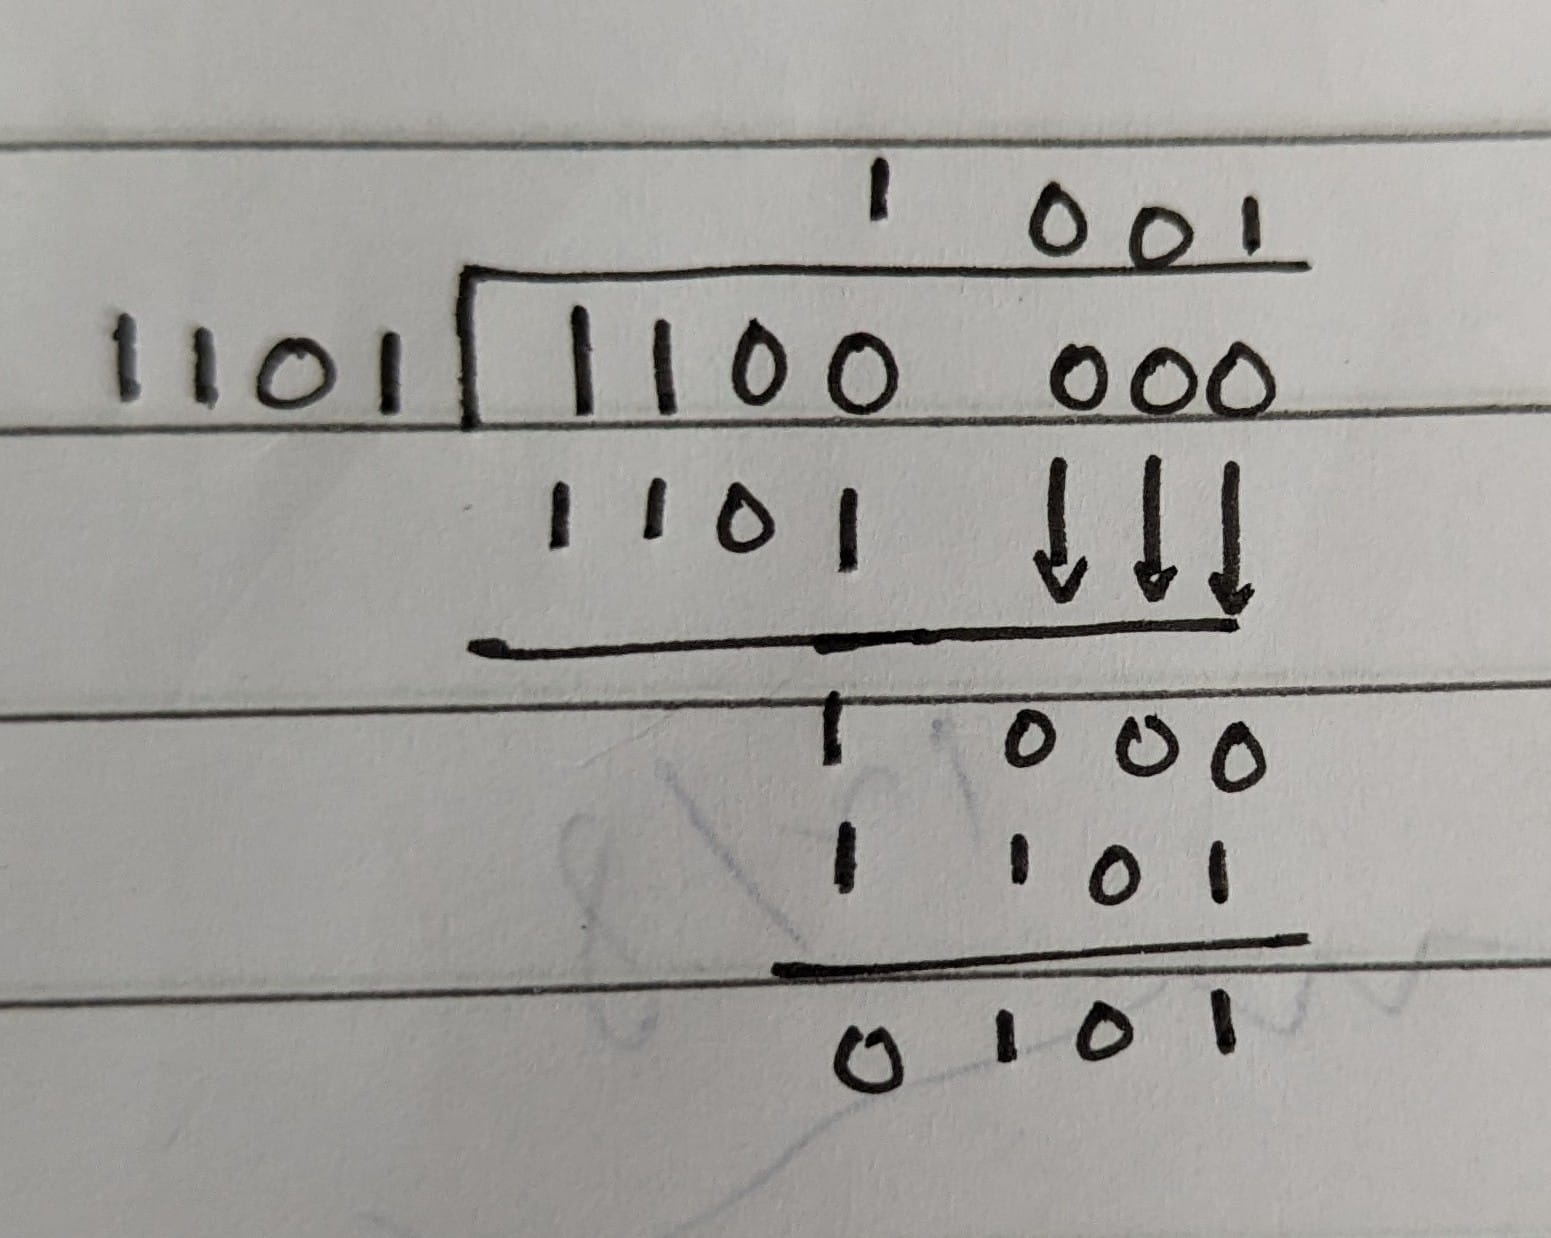
\includegraphics[scale = 0.1]{image2}
					\end{figure}
					\item Finally, we get our remainder as \textbf{$\mathbf{101}$}
				\end{enumerate}
				
				\part \textbf{How the DF and FCS look:}
				As per the given data specifications, the message will be:
				\begin{center}
					$\mathbf{1101\hspace{0.1 cm}101}$
				\end{center}
				\pagebreak
				\part \textbf{Remainder is $111$, is the message correct or not?}
				
				This question cannot be  properly answered. Modulo-2 division is non-invertible, meaning that simply having the remainder and the polynomial is not enough to reconstruct the message. Multiple possibilities exist from the remainder while back-tracking, meaning that we cannot determine whether the \textit{message} itself is unchanged.
				
				We can with certainty say that the entire bitstream has been changed, but we cannot make any comments on whether the message (in this case the letter) has been changed or not.
				
				\part \textbf{Suppose a bit flip happens. Can we correct with CRC? Mention alternatives}
				
				In the event of a bit-flip, CRC cannot find the exact location of the bit flip, only tell us whether or not it's happened. A better protocol to actually find out where the error occured would be to use something like a hamming code. As long as the number of bits in the message is a square number, we can apply a hamming code in order to both identify whether an error has occured and exactly where the error is.
		\end{parts}
		
		\newpage
		
		{\large \question \textbf{Unable to decode frequency}}
		
		\begin{parts}
			\part \textbf{Why?}\\
			The most likely reason is due to the doppler effect for the satellite in motion. There may also be equipment issues or electromagnetic field interference, causing this shift. (Although the electromagnetic field interference isn't too likely since Mars doesn't have a magnetic field).
			
			\part \textbf{Nature of this frequency offset from A to B.}
			
			At A, the frequency shift is positive, with the recieved frequency being higher than the transmitted one. At B, the frequency shift is negative. This occurs because at A, the satellite is moving towards the ground station and at B, the satellite is moving away.
			
			\part \textbf{Eliminate at hardware level.}
			
			The system described in the hint is known as a phase-locked loop(PLL) system. There are three parts, a voltage-controlled-oscillator which produces a signal who's frequency is dependent on the voltage used. The second piece is a phase detector that can measure the difference between the reference frequency and the output one. The change can be reapplied to the output until the reference and output frequency are the same.
		\end{parts} 
	\end{questions}
	
\end{document}